\documentclass{article}
\usepackage[utf8]{inputenc}
\usepackage{graphicx}
\usepackage{hyperref}
\hypersetup{
    colorlinks=true,
    linkcolor=blue,
    filecolor=magenta,      
    urlcolor=cyan,
}
\usepackage[total={6.0in, 10in}]{geometry}
\usepackage{multirow}
\usepackage{tabu}

\title{AML Final Project Proposal}
\author{Iris R. Seaman and Alesia Chernikova }
\date{}

\begin{document}

\maketitle

% Thing we want to do:
% \begin{enumerate}
%     \item change IWAE to IWAE-DReG
% \end{enumerate}

In our final project we will re-implement modules of \textit{Sequential Attend, Infer, Repeat: Generative Modelling of Moving Objects} (SQAIR) proposed by Adam R. Kosiorek et.al. which focuses on a vision problem of tracking objects in a sequence of images. The novelty in this papers lies in adding temporal dependencies between frames. By doing so, a variational auto-encoder learns to not only track objects, but as well as their dynamics throughout time. %This work is composed of two parts: Discovery and Propagation. Since the novelty lies in the Propogation part, our project will consist of  

SQAIR consists of two parts: Discovery and Propagation Inference. The Discovery part is responsible for detecting (or introducing, in the case of generation) new objects at every time-step, which is based on  AIR proposed by Eslami et.al. The Propagation Inference part updates (or forgets) latent variables from the previous time-step given the new observation (image).

The authors of the paper have provided a Github \href{https://github.com/akosiorek/sqair/blob/master/sqair/sqair_modules.py}{repository} of a Tensorflow implementation. For our final project, we propose a re-implementation of the Propagation Inference algorithm as seen in Figure~\ref{fig:prop}. Since the implementation requires several RNNs and further understanding of the code base, we hope to center our project on our understanding of the implementation. We will discuss our implementation in detail and follow-up with an in-depth discussion of the intuition behind the algorithm. By doing so, we hope to gain experience working with deep generative models, and state-of-the-art machine learning techniques. 

% We  will mainly deal with understanding the propagation inference part. We aim to do this by implementing it from scratch. While doing so, we will write our understanding of the implementation and include a discussion that describes why deep generative models make a difference in hard problems like object segmentation and tracking. Specifically, we will discuss why the implementation used specific neural networks as part of their models. 

The re-implementation will be in Tensorflow and we will train the Variational Autoencoder using two datasets, MNIST and DukeMTMC. Additionally, we will train the SQAIR using doubly reparameterized gradient estimator proposed by Tucker et.al. and compare the results. 


\begin{figure}[h]
\centering
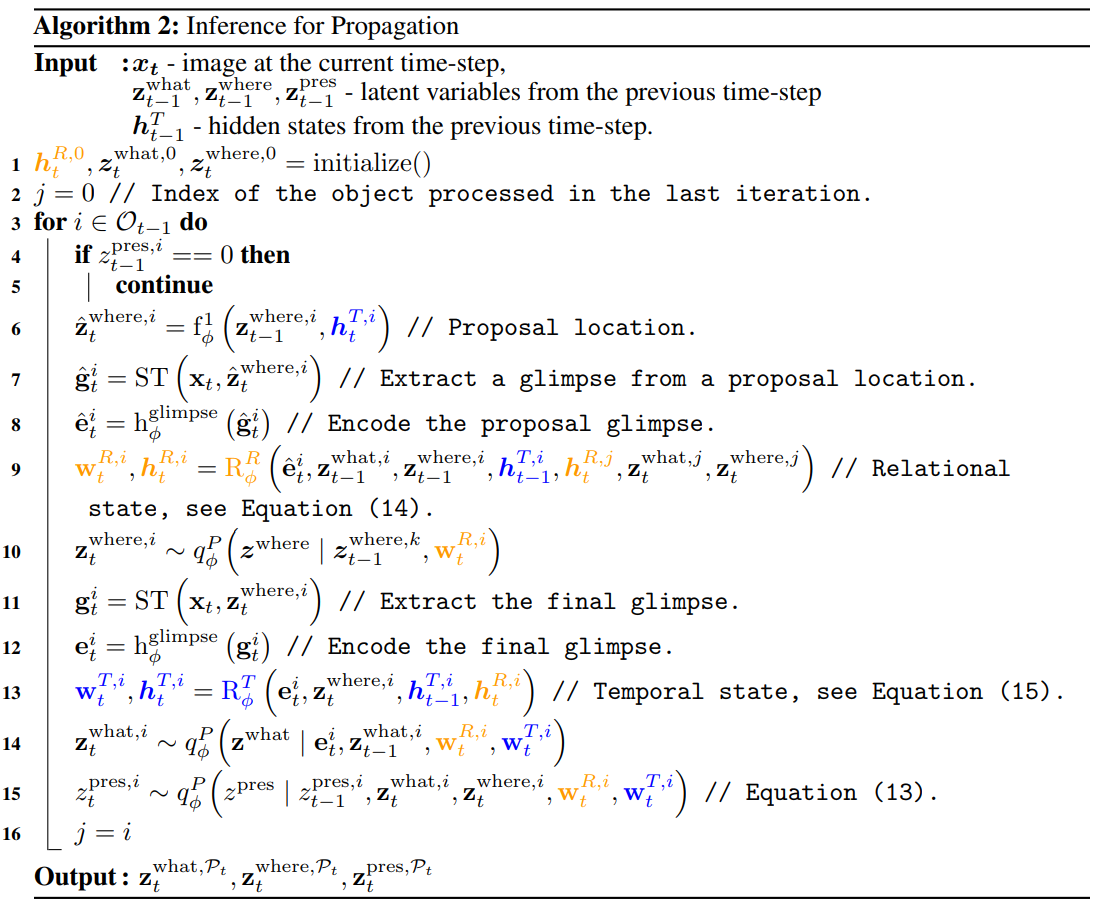
\includegraphics[width=5in]{prop.png}
\caption{Inference algorithm for Propagation}
\label{fig:prop}
\end{figure}


\newpage
% \section{Project Notes}

\textbf{April 11, 2019}

As part of the graph declaration for tensorflow, the object \texttt{SequentialAir} was instantiated. Inside \texttt{seq.py}, it begins by building all the nessessary params for tensor arrays for the tensorflow while loop call. This loop call is responsible for going through \textit{time}, $t=1:T$. For each time step we call our \texttt{SQAIRTimestep} object which is responsible for calling all of the inference and generative parts of propagate and discovery in order to calculate the log probabilities to later calculate the ELBO. We now discuss specific method implementation. 

\section{seq.py}
\subsection{SQAIRTimestep: \_build}


\begin{center}
\begin{tabular}{ | m{10em} | m{12cm}| } 
\hline
Parameter& Description \\ 
\hline
 img & Tensor of size [B, H, W, C] representing images \\ 
\hline
 z\_tm1 &   4-tuple of [what, where, presence, presence\_logit] from previous time-step.\\ 
\hline
temporal\_hidden\_state & Hidden state of the time\_cell \\
\hline
prop\_prior\_state & Hidden state of the propagation prior. \\
\hline
highest\_used\_ids & Integer Tensor of size [B], where each entry represent the highest used object
            ID for the corresponding data example in the batch. \\
\hline
prev\_ids & Integer Tensor of size [B, n\_steps], with each entry representing object ID of the
            corresponding object at the previous time-step. \\
\hline
time\_step & Integer \\
\hline
\hline
\hline
\end{tabular}
\end{center}

The first call inside \_build is to get the outputs from \texttt{propagation} and \texttt{discovery}. 

So now we move on that method.

\subsubsection{SQAIRTimestep: \_propagate\_and\_discover}


\subsection{Propagate: \_build}
\begin{center}
\begin{tabular}{ | m{10em} | m{12cm}| } 
\hline
Parameter& Description \\ 
\hline
 img & Tensor of size [B, H, W, C] representing images \\ 
\hline
 z\_tm1 &   4-tuple of [what, where, presence, presence\_logit] from previous time-step.\\ 
\hline
temporal\_hidden\_state & Hidden state of the time\_cell \\
\hline
prop\_prior\_state & Hidden state of the propagation prior. \\
\hline
\end{tabular}
\end{center}

Propagate requires running our generative and inference model in order to compute log probabilities. In order to run our generative model, we need to call our prior. 

\section{propagate.py}

\subsection{PropagatePrior: \_build}

\begin{center}
\begin{tabular}{ | m{10em} | m{12cm}| } 
\hline
\textbf{Parameter}& \textbf{Description} \\ 
\hline
 z\_tm1 &   4-tuple of [what, where, presence, presence\_logit] from previous time-step.\\ 
\hline
prior\_rnn\_hidden\_state & Hidden state of the propagation prior. \\
\hline
\end{tabular}
\end{center}

\end{document}
